\chapter{Methods}


\textit{\textendash\ ``Open the gates now. Private, lower your weapon''. \\ 
\textendash\ ``Not till we feed these people. Court martial me, sir. Do whatever you want with me but not till those people are fed''.\\
\textemdash\ ``Black 47'' by Lance Daly}	
	
\section{Generalized Additive Model}

Due to the difficulty in capturing the non-linear relationship, it is necessary to use scatter plots to observe what the non-linear relationship between the independent and dependent variables is. Figure 4.1 provides an overview of the relationship between independent and dependent variables. The three scatter plots in the first column represent three sets of independent and dependent variables with significant linear relationships, while the three scatter plots in the second column represent three sets of non-significant linear, or non-linear, relationships.

Based on the theory of the entitlement approach mentioned earlier, it is indeed possible that there is a non-linear relationship between the independent and dependent variables, for example, when the price of cereals rises marginally, farmers may grow as a result of this profit, whereas when the price of cereals rises significantly, the farmers' trade-base entitlement is consequently jeopardized, and the population of the year ends up declining. According to this logic, linear regression is not a very good choice here and it is necessary to take other forms of non-linear regression for analysis.

\begin{figure}[htbp]
    \centering
    \caption{Regression Scatter}
    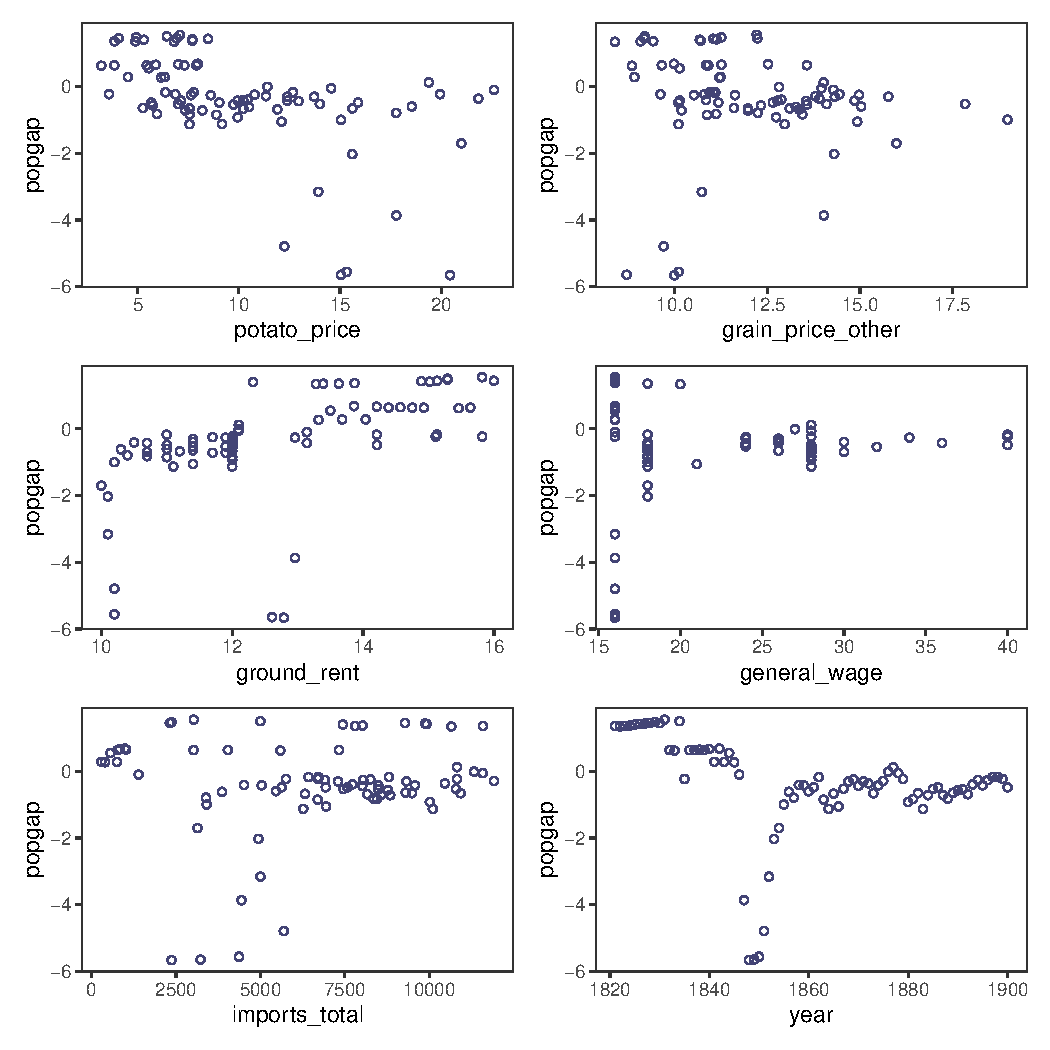
\includegraphics[width=.95\textwidth]{../03_outputs/regression_scatter.pdf}
\end{figure}

Hello

\section{Research Framework}
\begin{landscape}
    \begin{figure}[htbp]
        \centering
        \caption{Research Framework}
        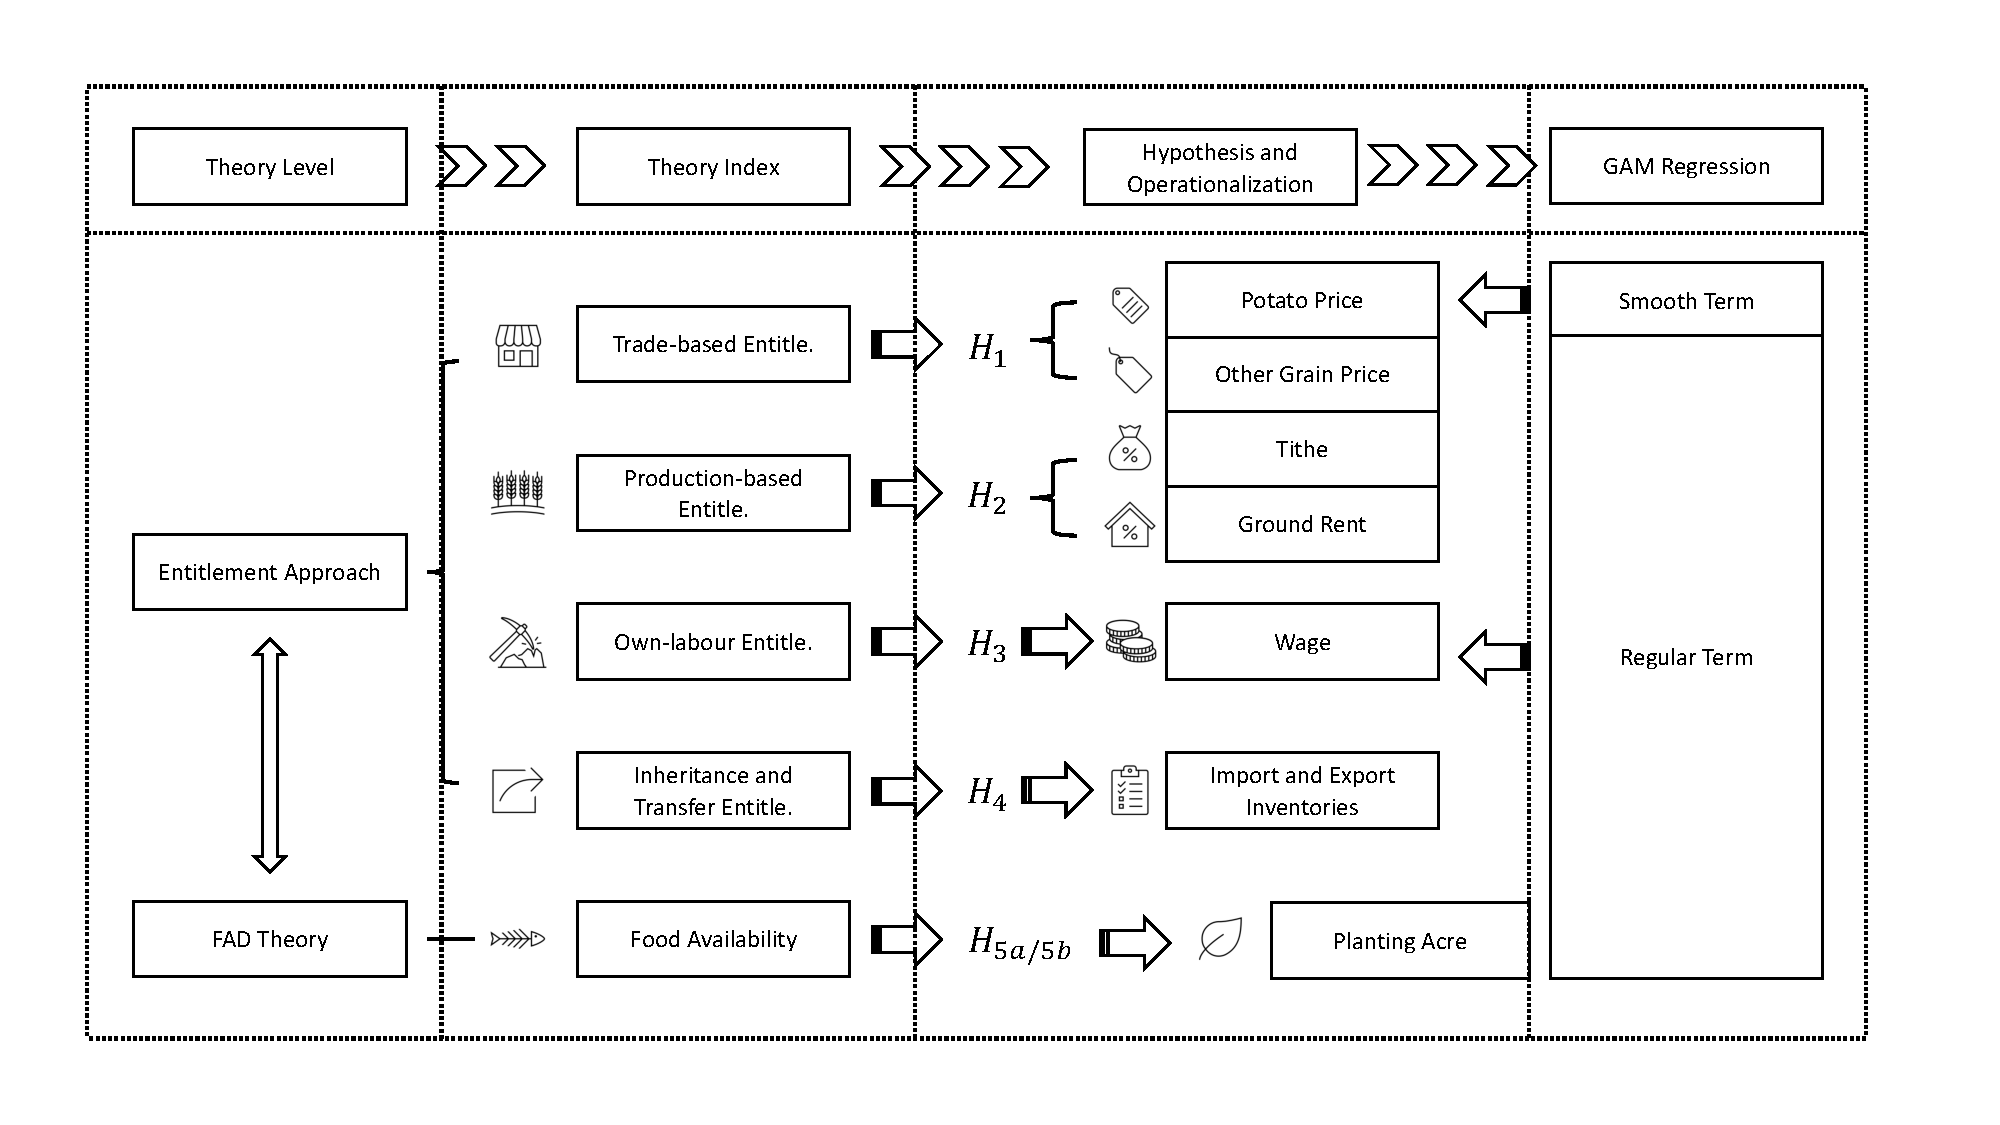
\includegraphics[width=1.5\textheight]{../03_outputs/Framework.pdf}
    \end{figure}
\end{landscape}

\section{Replication}
